				\documentclass[10pt,a4paper]{article}
				\usepackage[english]{babel}
				\usepackage[utf8]{inputenc}
				\usepackage{fancyhdr}
				\usepackage{hyperref}
				\usepackage{graphicx}
				\usepackage{subcaption}
				\usepackage{caption}
				\usepackage{cite}
				\usepackage{booktabs}
				\usepackage{wrapfig}
				\usepackage{float}
				\usepackage{amsmath}
				\usepackage{xcolor}
				\usepackage{listings}
				\lstset{
					basicstyle=\ttfamily,
					columns=fullflexible,
					frame=single,
					breaklines=true,
					%postbreak=\mbox{\textcolor{red}{$\hookrightarrow$}\space},
				}
				
				\restylefloat{table}
			
				\pagestyle{fancy}
				\fancyhf{}
				\rhead{\today}
				\lhead{Assignment 05}
				\rfoot{Page \thepage}
			
				\begin{document}
				\begin{titlepage}
				\centering
			
					{\scshape\LARGE Scientific Experimentation and Evaluation\par}
			
					{\scshape\Large Assignment: 06\par}
			
					\vfill
			
					\vfill
					{\Large\itshape Anees Khan (9030423)
						\\Debaraj Barua (9030412)\\
						Md Zahiduzzaman (9030432)
						\par}
					\vfill
			
					{\large 14-June-2018\par}
				\end{titlepage}
				\tableofcontents
				\listoffigures	
				\listoftables
				\newpage
				\section{Relevant Aspects of Experiment}
				\subsection{Apparatus}
					\subsubsection{Hardware}
						\begin{itemize}
							\item KUKA youBot arm \textcolor{blue}{(Number: 1)}.
							\item Objects of three different sizes and weights, with ArUco markers attached to the top.
							\item Camera (Microsoft LifeCam).
							\item Two computers, one to run the robot and other for data gathering from the camera.
							\item A fixed container or marker on the table to ensure that the initial object position is kept constant.
						\end{itemize}
					\subsubsection{Software and Libraries used}
						\begin{itemize}
							\item KUKA youBot drivers.
							\item Control scripts for the arm to pick and move the objects in one of the three predefined placing poses.
							\item Marker pose subscribed script, to gather pose of the object.
							\item \textbf{LibreOffice Calc} for data management.
							\item \textbf{Python} for data visualization and calculations
							\item Python libraries:
							\begin{itemize}
								\item pandas
								\item numpy
								\item matplotlib
								\item seaborn
								\item scipy.stats
							\end{itemize}
							\end{itemize}		
											
				\subsection{Procedure}	
					\begin{itemize}
						\item First we run the script to get the arm in the pre-grasp position.
						\item We then place the object in the container, keeping the marker's orientation constant throughout the experiment.\\
						\item We then run the script to move the arm in one of the three pre-defined positions; and repeat this twenty times for each weight and pose combination. Thus, giving us 180 readings of pose coming from three different objects in three different orientations.
						\item Once the object is placed and the arm moves back to a stationary position, we run the subscriber script to collect pose readings of 50 frames from the camera. This is repeated after each motion.
					\end{itemize}
				\subsection{Expected Problems and Performance}
					\begin{itemize}
						\item The picking position of the arm might differ from the ground truth, because of vibrations, motion in the table and a variety of other physical conditions.
						\item The placement of the object in the container might not always be aligned properly.
						\item The marker on top of the object might move during movement and thus will lead to improper pose data.
						\item After placing the object, the gripper might touch it while moving away, which will introduce distortions in \textcolor{blue}{orientation} data.
						\item The light might not always be uniform, which might also cause some improper readings.						
					\end{itemize}
					
				\section{Observations and Data}
					 \subsection{Visualization}
						 \subsubsection{\textcolor{blue}{Data Visualization}}
						\begin{itemize}
							\item The raw data with fifty reading for each run has been filtered and saved as an average. This data is used for further visualization. 
							\item In addition to this, data shared by other groups using the same arm has been included to get a sample size of 180 pose readings in each direction.
							\item The first visualization shows the pose distribution of large, medium and small objects in three directions including the initial and expected pose. 
							\item The upper right hand corner is the left run plot and the lower left hand corner is right run plot.
							\begin{figure}[h]
								\centering
								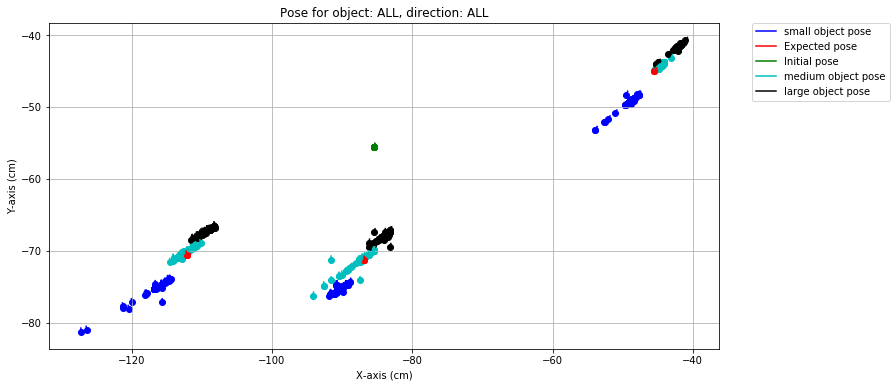
\includegraphics[width=1.0\linewidth]{img/pose_all_all.png}
								\caption{poses for all objects in straight, left and right direction}
								\label{fig:poses for all objects in straight, left and right direction}
							\end{figure}
					\end{itemize}			
	    				 \subsubsection{Outlier Detection And Removal From Raw Data}
	    				 \begin{itemize}
	    				 	\item We filtered the noisy raw data by removing all records with x, y or theta value outside the range of $\mu_x \pm 2\sigma_x$, $\mu_y \pm 2\sigma_y$, $\mu_\theta \pm 2\sigma_\theta$ respectively. We used the filtered raw data to calculate mean for each experimental trial. Total number of outlier is 495 and outlier per experimental run is 2.75
	    				 	%\item \textcolor{red}{Filter oulier from all data}\\
	    				 \end{itemize}
		    				 
						 \subsubsection{\textcolor{blue}{Pose Visualization}}
%							\begin{itemize}
%								\item The first section shows the pose plots of small, medium and large objects in straight path. 
%								\item It shows the initial pose, the expected(ground truth) and observed pose(twenty points).  
%								\item The same process is repeated for left followed by right run.
								
								\begin{figure}[H]
%									\begin{subfigure}{0.5\textwidth}
%										\centering
%										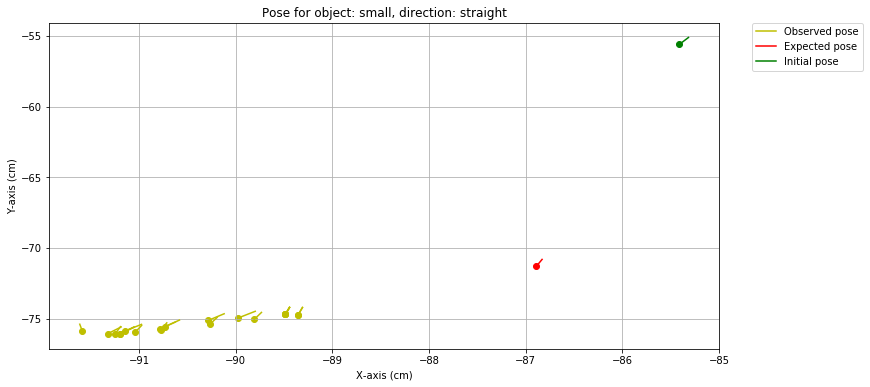
\includegraphics[width=0.8\linewidth]{img/pose_small_straight.png}
%										\caption{object: small, direction: straight}
%										\label{fig:object: small, direction: straight}
%									\end{subfigure}%
%									\begin{subfigure}{0.5\textwidth}
%										\centering
%										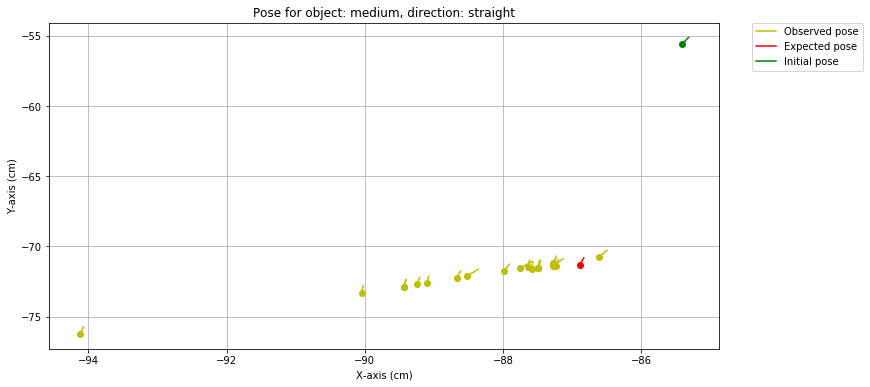
\includegraphics[width=0.8\linewidth]{img/pose_medium_straight.png}
%										\caption{object: medium, direction: straight}
%										\label{fig:object: medium, direction: straight}
%									\end{subfigure}
%									
%									\begin{subfigure}{0.5\textwidth}
%										\centering
%										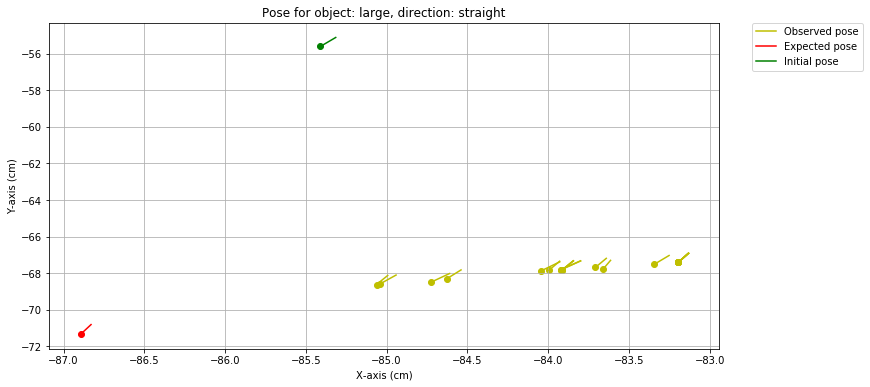
\includegraphics[width=0.8\linewidth]{img/pose_large_straight.png}
%										\caption{object: large, direction: straight}
%										\label{fig:object: large, direction: straight}
%									\end{subfigure}%
									
									\begin{subfigure}{\textwidth}
										\centering
										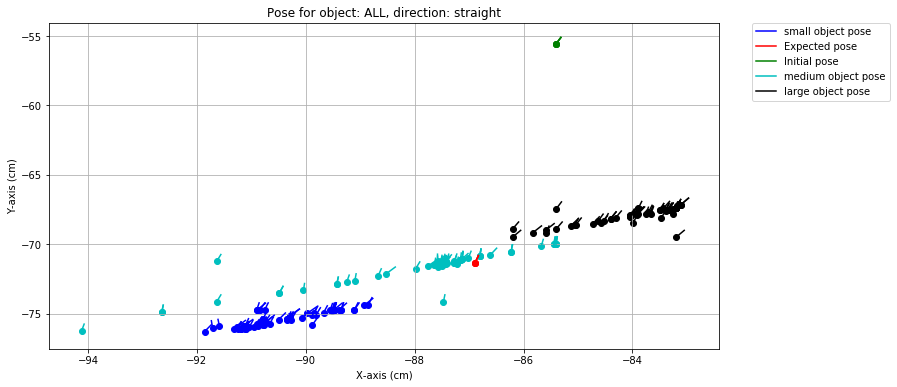
\includegraphics[width=0.8\linewidth]{img/pose_all_straight.png}
										\caption{object: all, direction: straight}
										\label{fig:object: all, direction: straight}
									\end{subfigure}
									
									\caption{pose in straight direction}
									\label{fig:pose in straight direction}
								\end{figure}
								
								\begin{figure}[H]
%									\begin{subfigure}{0.5\textwidth}
%										\centering
%										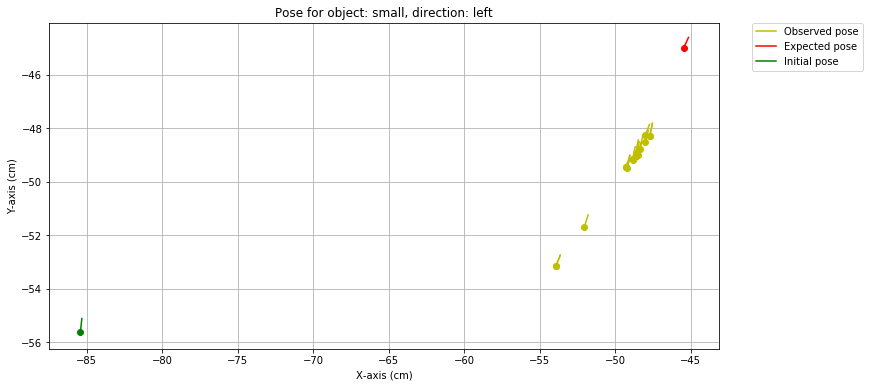
\includegraphics[width=0.8\linewidth]{img/pose_small_left.png}
%										\caption{object: small, direction: left}
%										\label{fig:object: small, direction: left}
%									\end{subfigure}%
%									\begin{subfigure}{0.5\textwidth}
%										\centering
%										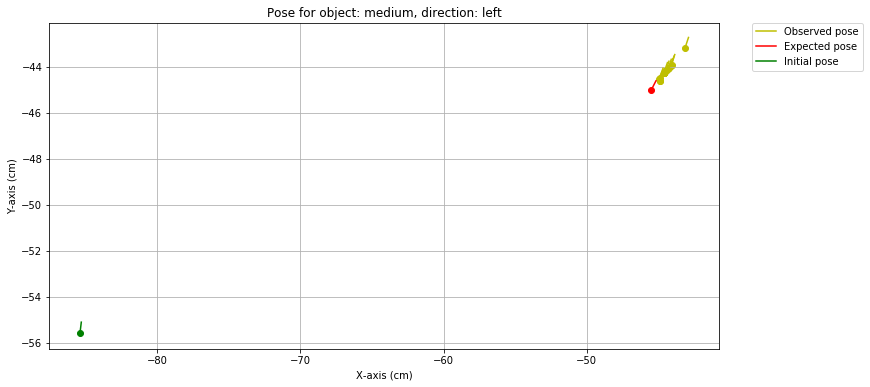
\includegraphics[width=0.8\linewidth]{img/pose_medium_left.png}
%										\caption{object: medium, direction: left}
%										\label{fig:object: medium, direction: left}
%									\end{subfigure}
%									
%									\begin{subfigure}{0.5\textwidth}
%										\centering
%										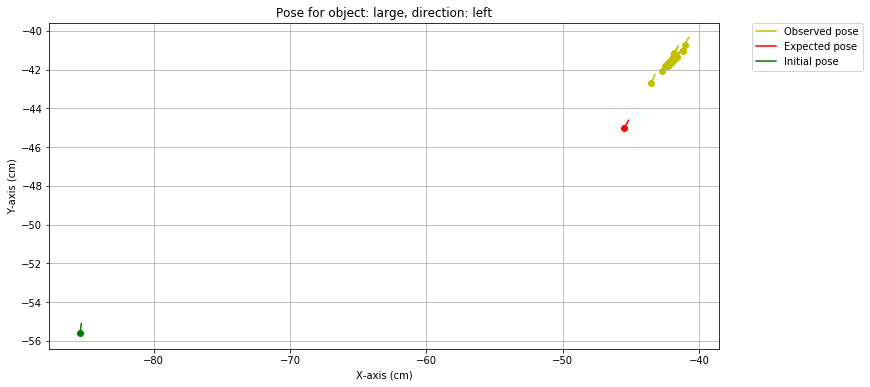
\includegraphics[width=0.8\linewidth]{img/pose_large_left.png}
%										\caption{object: large, direction: left}
%										\label{fig:object: large, direction: left}
%									\end{subfigure}%
									\begin{subfigure}{\textwidth}
										\centering
										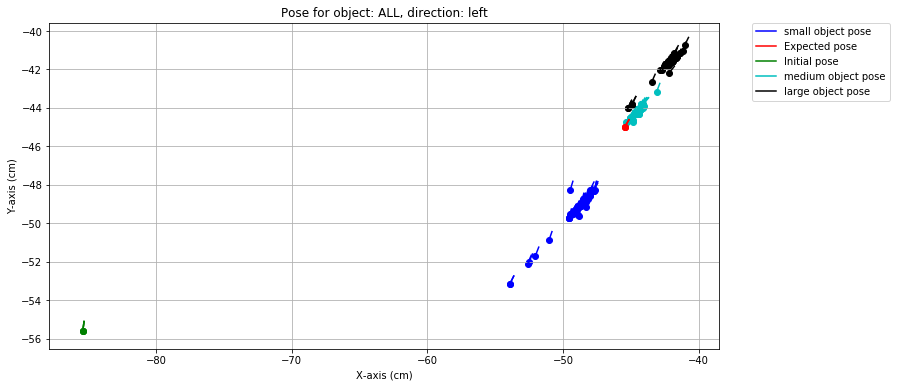
\includegraphics[width=0.8\linewidth]{img/pose_all_left.png}
										\caption{object: all, direction: left}
										\label{fig:object: all, direction: left}
									\end{subfigure}
									
									\caption{pose in left direction}
									\label{fig:pose in left direction}
								\end{figure}
								
								\begin{figure}[H]
%									\begin{subfigure}{0.5\textwidth}
%										\centering
%										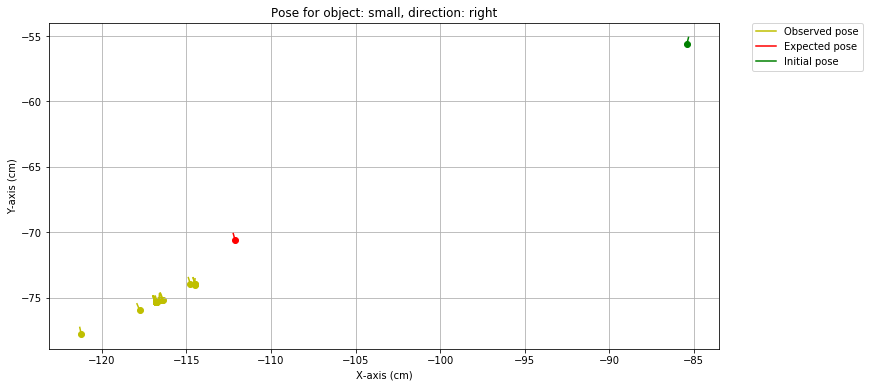
\includegraphics[width=0.8\linewidth]{img/pose_small_right.png}
%										\caption{object: small, direction: right}
%										\label{fig:object: small, direction: right}
%									\end{subfigure}%
%									\begin{subfigure}{0.5\textwidth}
%										\centering
%										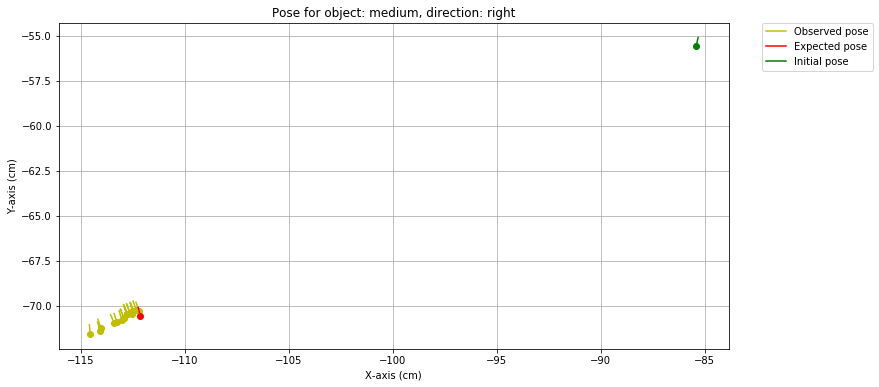
\includegraphics[width=0.8\linewidth]{img/pose_medium_right.png}
%										\caption{object: medium, direction: right}
%										\label{fig:object: medium, direction: right}
%									\end{subfigure}
%									
%									\begin{subfigure}{0.5\textwidth}
%										\centering
%										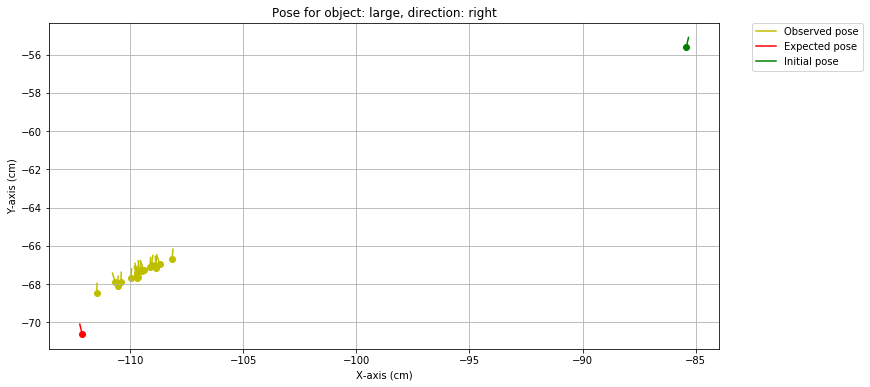
\includegraphics[width=0.8\linewidth]{img/pose_large_right.png}
%										\caption{object: large, direction: right}
%										\label{fig:object: large, direction: right}
%									\end{subfigure}%
									\begin{subfigure}{\textwidth}
										\centering
										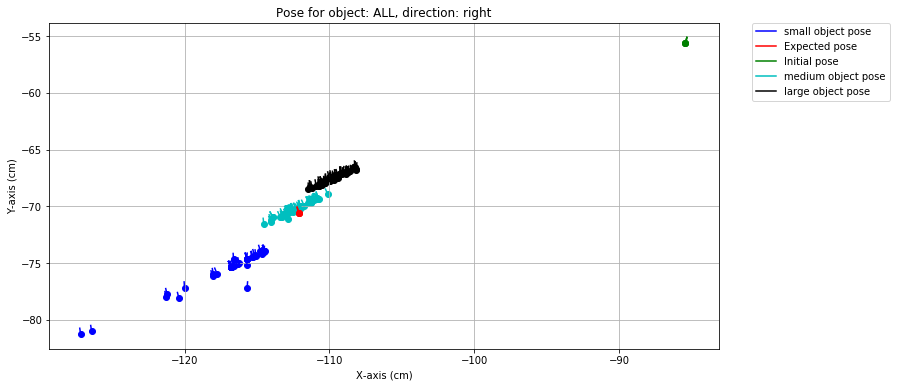
\includegraphics[width=0.8\linewidth]{img/pose_all_right.png}
										\caption{object: all, direction: right}
										\label{fig:object: all, direction: right}
									\end{subfigure}
									
									\caption{pose in right direction}
									\label{fig:pose in right direction}
								\end{figure}

%							\end{itemize}	
					
				\section{\textcolor{blue}{Results}}
					\subsection{Final Position \& Accuracy }
						\subsubsection{Numerical Results}
							\begin{table}[H]
\centering
\caption{Ground Truth}
\label{groundTruth}
\begin{tabular}{|l|c|c|c|}
\hline
\multicolumn{1}{|c|}{Direction} & X (cm)  & Y (cm) &  $\theta$ (radians) \\ \hline
Straight                        & -86.89  & -71.31 & 1.45            \\ %\hline
Left                            & -45.47  & -45.00 & 0.88            \\ %\hline
Right                           & -112.13 & -70.58 & 1.78            \\ \hline
\end{tabular}
\end{table}

							\begin{table}[H]
\centering
\caption{Final Pose along straight direction}
\label{straight}
\begin{tabular}{|l|c|c|c|}
	\hline
	\multicolumn{1}{|c|}{Object Type} & X (cm) & Y (cm) &  $\theta$ (radians)   \\ \hline
	Small                             & -90.34 & -75.31 & 1.40				    \\ %\hline
	Medium                            & -87.85 & -71.63 & 1.48				    \\ %\hline
	Large                             & -84.00 & -67.94 & 1.39    				\\ \hline
	Combined                          & -87.40 & -71.63 & 1.42				    \\ \hline
\end{tabular}
\end{table}

							\begin{table}[H]
\centering
\caption{Final pose along left direction}
\label{left}
\begin{tabular}{|l|c|c|c|}
	\hline
	\multicolumn{1}{|c|}{Object Type} & X (cm) & Y (cm) &  $\theta$ (radians)	\\ \hline
	Small                             & -49.14 & -49.38 & 1.05				    \\ %\hline
	Medium                            & -44.52 & -44.19 & 0.88    				\\ %\hline
	Large                             & -42.25 & -41.73 & 0.88    				\\ \hline
	Combined                          & -45.30 & -45.10 & 0.93    				\\ \hline
\end{tabular}
\end{table}

							\begin{table}[H]
\centering
\caption{Final pose along right direction}
\label{right}
\begin{tabular}{|l|c|c|c|}
	\hline
	\multicolumn{1}{|c|}{Object Type} & X (cm)  & Y (cm) & $\theta$ (radians) \\ \hline
	Small                             & -116.76 & -75.35 & 1.72    			  \\ %\hline
	Medium                            & -112.28 & -70.20 & 1.83           	  \\ %\hline
	Large                             & -109.68 & -67.46 & 1.62    			  \\ \hline
	Combined                          & -112.93 & -71.03 & 1.72    			  \\ \hline
\end{tabular}
\end{table}

						\subsubsection{Accuracy}
						\begin{itemize}
							\item Straight Run:
							\begin{itemize}
								\item Standard Deviation Straight: [2.89 3.13 0.09]
								\item Accuracy in X:  99.42
								\item Accuracy in Y:  99.56
								\item Accuracy in theta:  98.06								
							\end{itemize}
							
							\item Left Run:
							\begin{itemize}
								\item Standard Deviation Left: [3.00 3.26 0.17]
								\item Accuracy in X:  99.62
								\item Accuracy in Y:  99.80
								\item Accuracy in theta:  93.83								
							\end{itemize}
							
							\item Right Run:
							\begin{itemize}
								\item Standard Deviation Left: [3.32 3.40 0.146]
								Accuracy in X:  99.28
								Accuracy in Y:  99.37
								Accuracy in theta:  96.91								
							\end{itemize}
						
						\end{itemize}
					\subsection{Compare Data with Gaussian}
%					To verify if the observed data follows a gaussian distribution, we use a the \textit{scipy} library. The \textit{scipy.stats.normaltest} function is used to check if the data follows a normal distribution. 
%					
%					We observe that the threshold value of $p$ value is more than $0.05$,indicating that the data is normally distributed.
%					
%					However, for the right arc motion, we see that the data observed do not follow a Gaussian distribution, this can be attributed to some outlying data points. The reason for these data points has been explored in the expected problems and performance section.
					
					\begin{figure}[H]
						\begin{subfigure}{\textwidth}
							\centering
							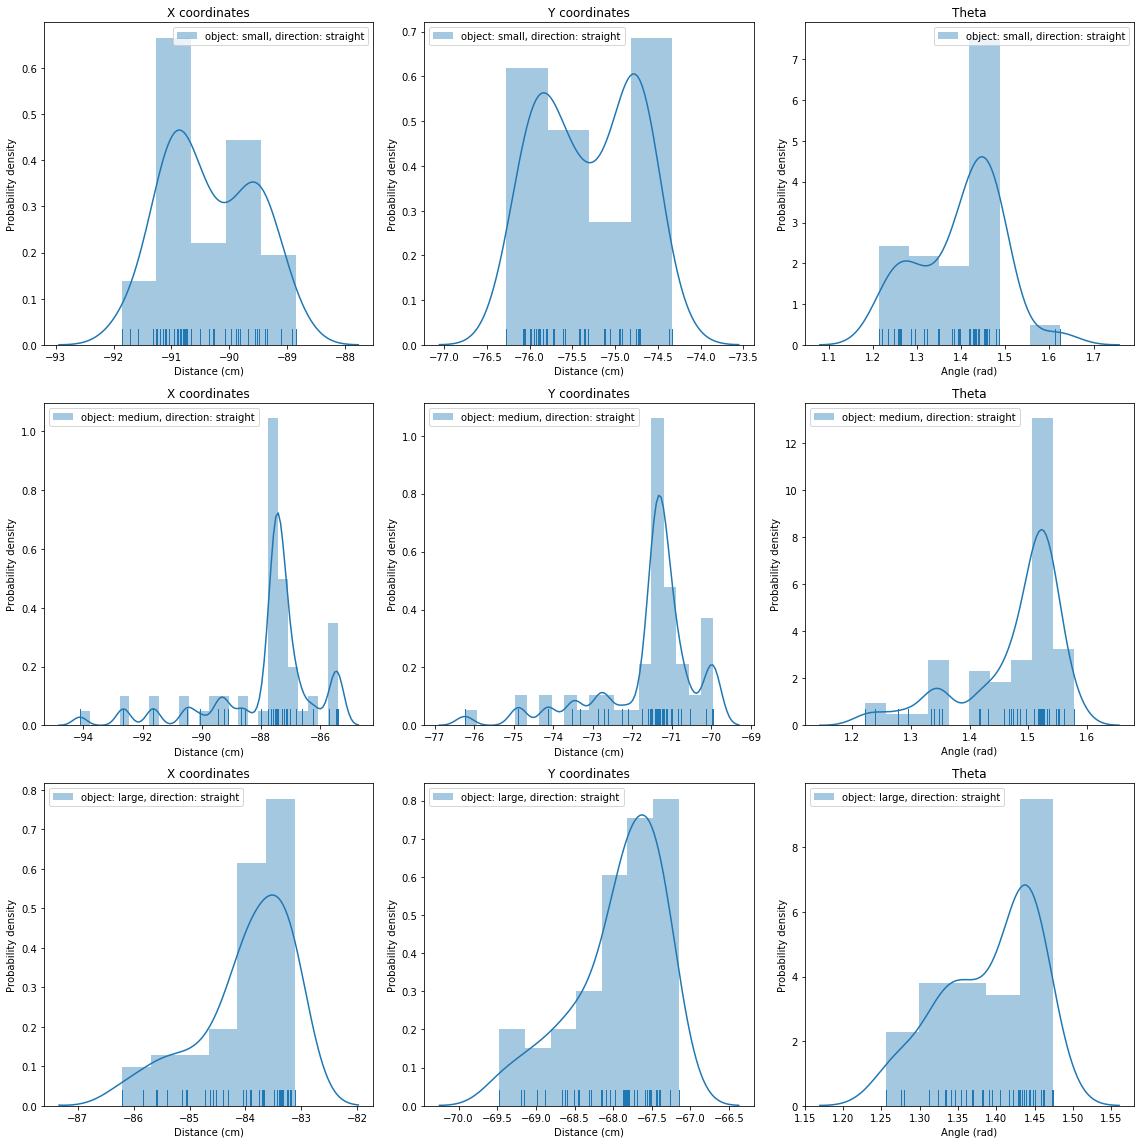
\includegraphics[width=\linewidth]{img/st_hist.png}							
						\end{subfigure}
						\begin{subfigure}{\textwidth}
							\centering
							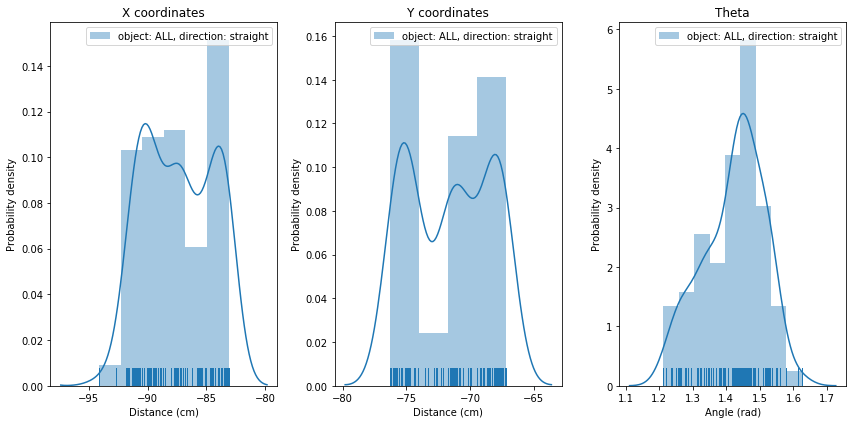
\includegraphics[width=\linewidth]{img/st_hist_combined.png}
						\end{subfigure}
						\caption{Histogram and Gaussian distribution of data for straight run}
					\end{figure}
					\begin{figure}[H]
						\begin{subfigure}{\textwidth}
							\centering
							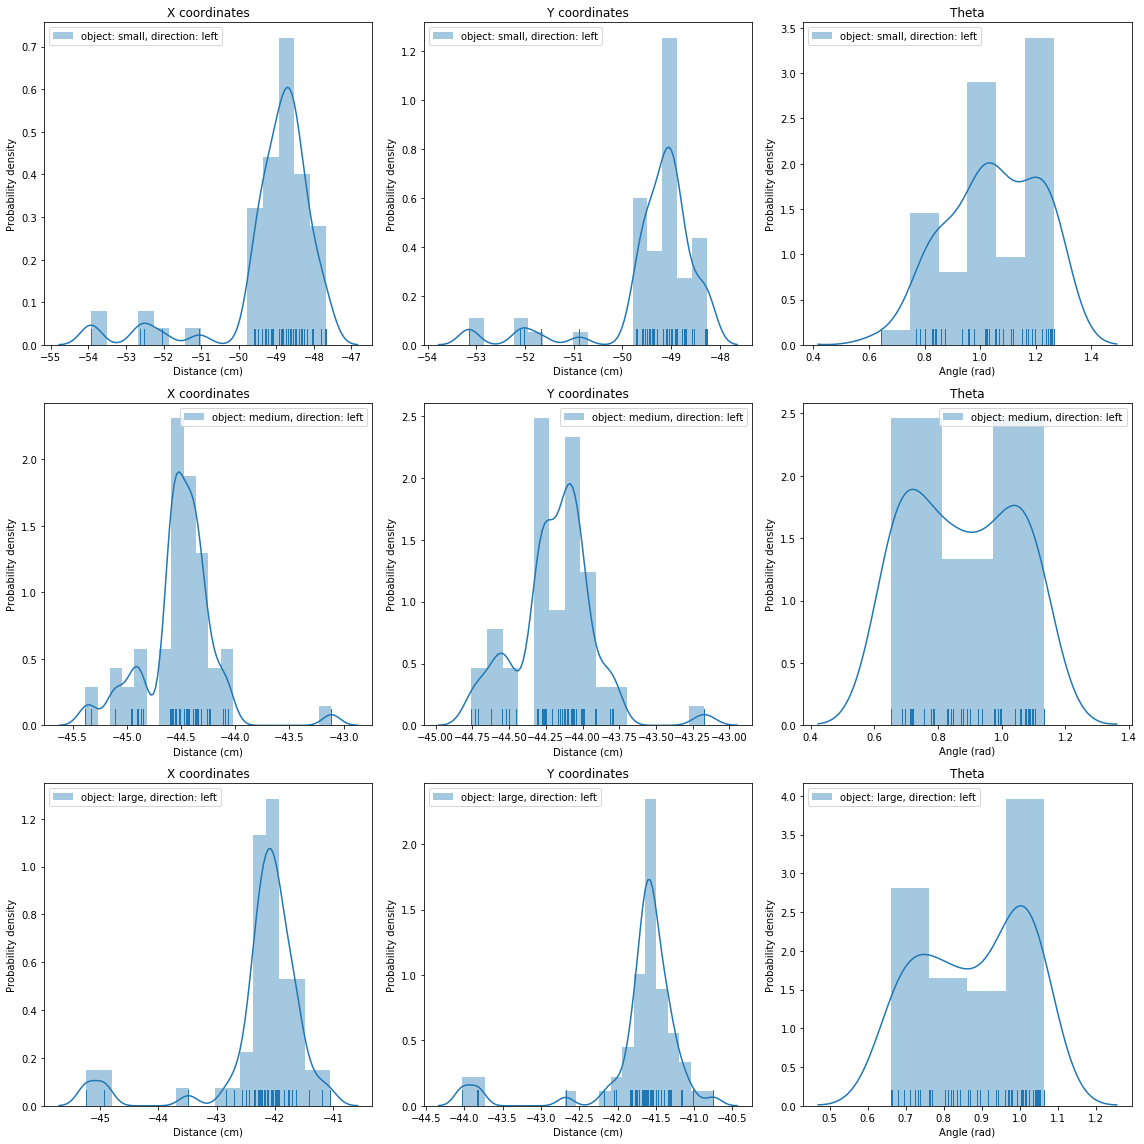
\includegraphics[width=\linewidth]{img/left_hist.png}						
						\end{subfigure}
						\begin{subfigure}{\textwidth}
							\centering
							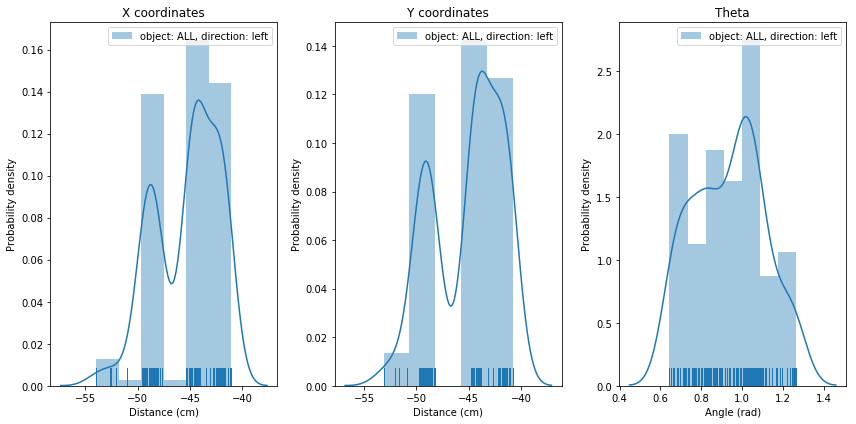
\includegraphics[width=\linewidth]{img/left_hist_combined.png}				
						\end{subfigure}
						\caption{Histogram and Gaussian distribution of data for left run}
					\end{figure}
					\begin{figure}[H]
						\begin{subfigure}{\textwidth}
							\centering
							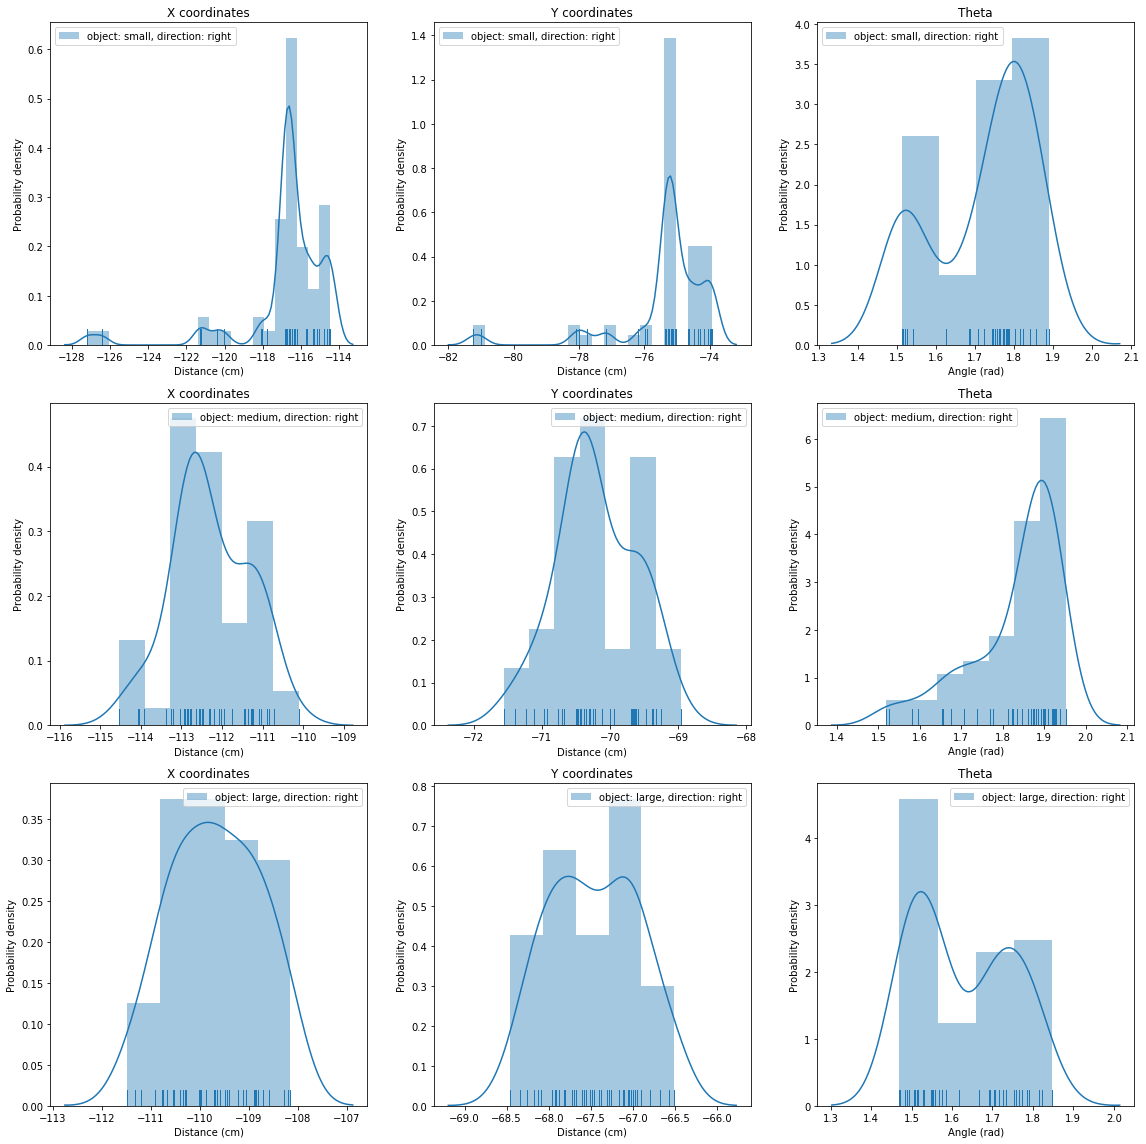
\includegraphics[width=\linewidth]{img/right_hist.png}
						\end{subfigure}
						\begin{subfigure}{\textwidth}
							\centering
							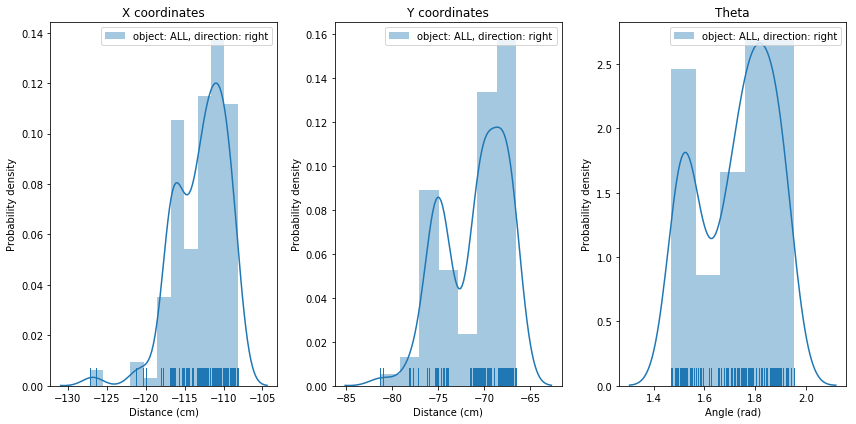
\includegraphics[width=\linewidth]{img/right_hist_combined.png}
						\end{subfigure}
						\caption{Histogram and Gaussian distribution of data for right run}
					\end{figure}
					\subsection{Outlier Removal and Hypothesis Testing}
						\begin{itemize}
							\item Outliers are calculated on the basis of Z-Score, as per below:
							$$Z = \frac{x-\mu_0}{\frac{\sigma}{\sqrt{n}}}$$
							Here, $\mu_0$ represents the ground truth,\\
							$x$ is the data point in consideration,\\
							$\sigma$ is the standard deviation of the observed data, and\\
							$n$ represents the sample size.
							\item Using the above formula, we iterate over all the data points, and remove any entry where the absolute $Z$ value is greater than a critical value of $3.819$.
							\item The limit is selected on the basis of a confidence value of $(1-\alpha) = 0.9999$ \cite{hypothesisTesting}							
							\item An example for this is given below:
								\begin{figure}[H]
									\begin{subfigure}{\textwidth}
										\centering
										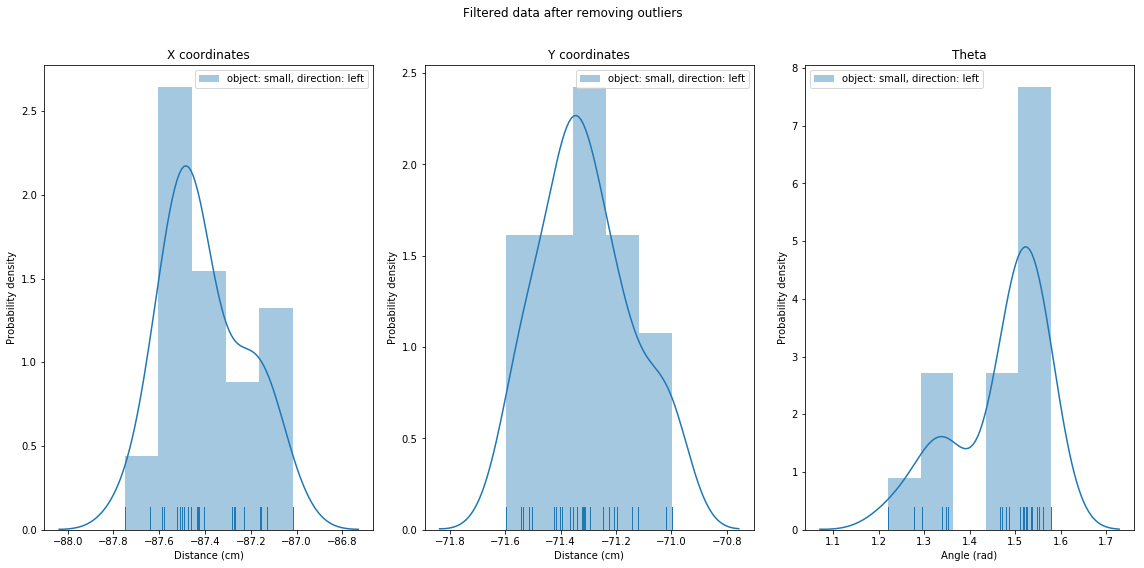
\includegraphics[width=\linewidth]{img/filtered/small_left_filtered.png}				
									\end{subfigure}
									\begin{subfigure}{\textwidth}
										\centering
										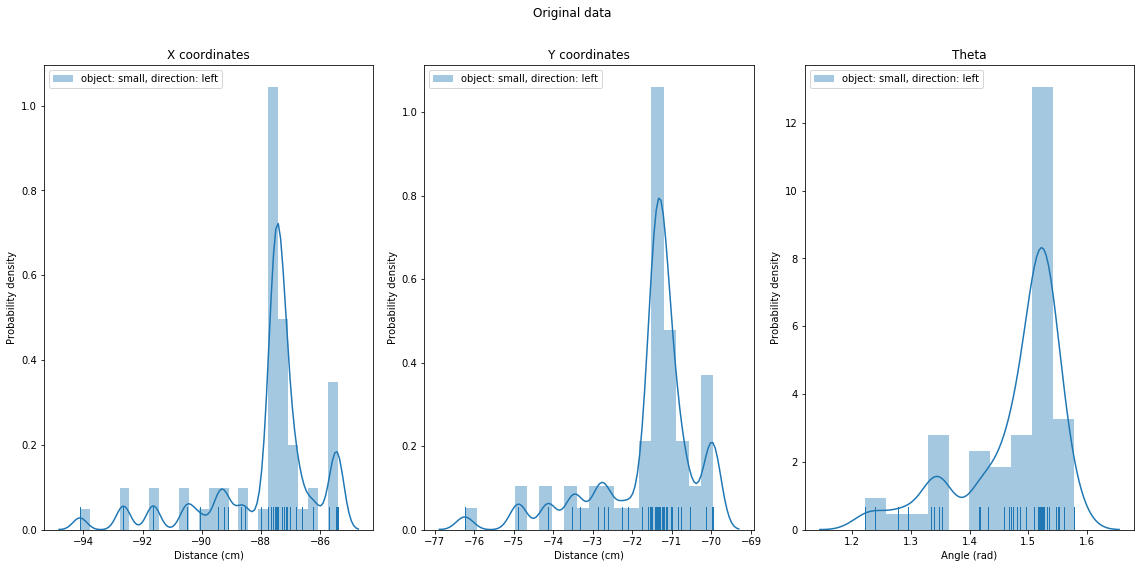
\includegraphics[width=\linewidth]{img/filtered/small_left_org.png}
									\end{subfigure}
									\caption{Outlier removal on small object and left run}
								\end{figure}
						\end{itemize}
						
%						\begin{figure}[H]
%							\begin{subfigure}{\textwidth}
%								\centering
%								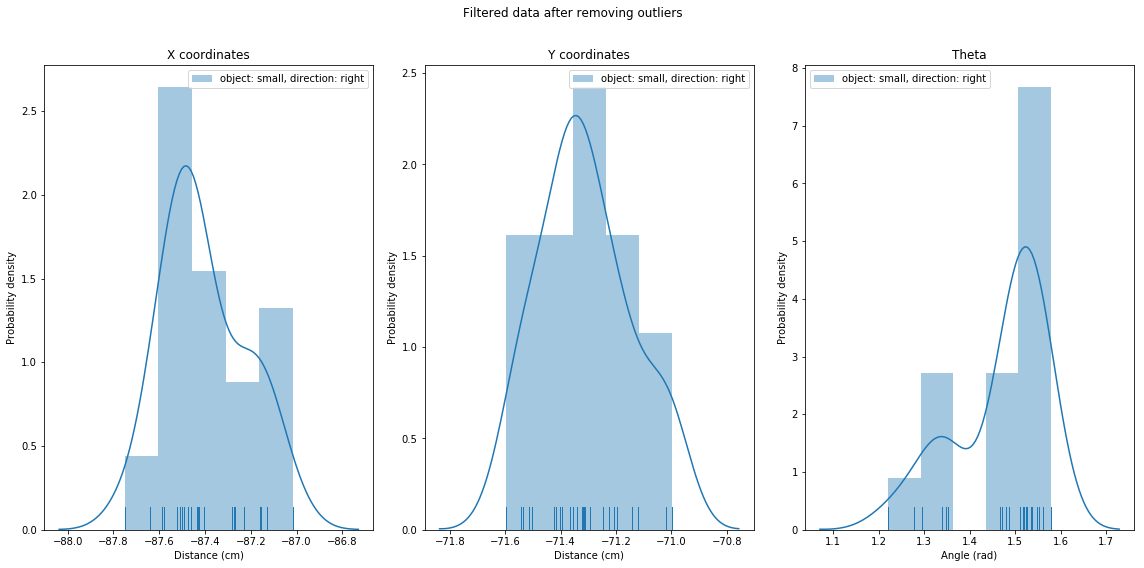
\includegraphics[width=\linewidth]{img/filtered/small_right_filtered.png}				
%							\end{subfigure}
%							\begin{subfigure}{\textwidth}
%								\centering
%								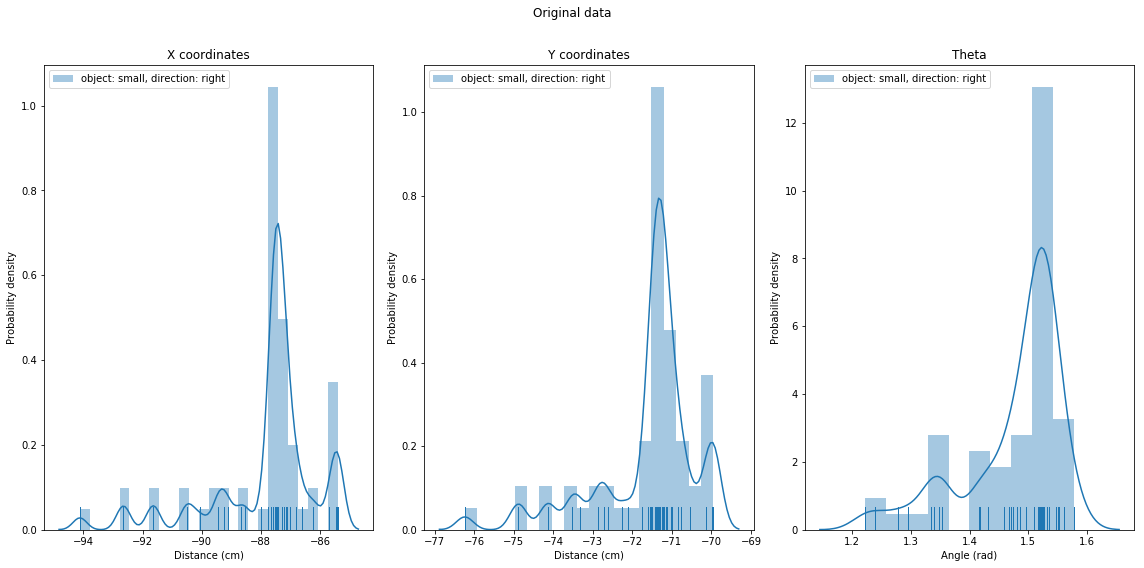
\includegraphics[width=\linewidth]{img/filtered/small_right_org.png}
%							\end{subfigure}
%							\caption{Outlier removal on small object and right run}
%						\end{figure}
%						\begin{figure}[H]
%							\begin{subfigure}{\textwidth}
%								\centering
%								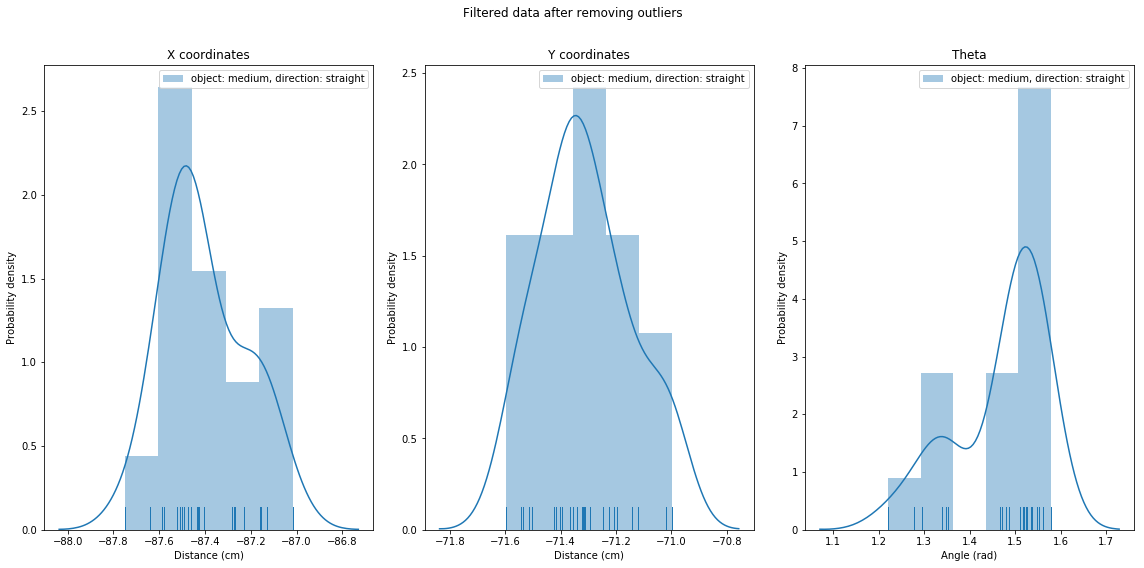
\includegraphics[width=\linewidth]{img/filtered/medium_st_filtered.png}				
%							\end{subfigure}
%							\begin{subfigure}{\textwidth}
%								\centering
%								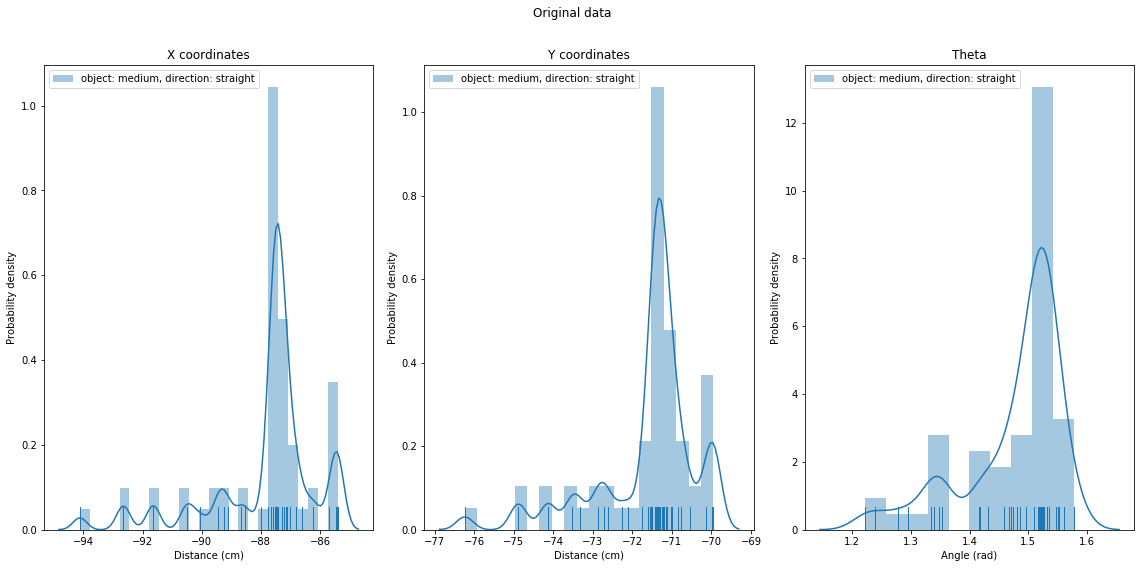
\includegraphics[width=\linewidth]{img/filtered/medium_st_org.png}
%							\end{subfigure}
%							\caption{Outlier removal on medium object and straight run}
%						\end{figure}	
%						\begin{figure}[H]
%							\begin{subfigure}{\textwidth}
%								\centering
%								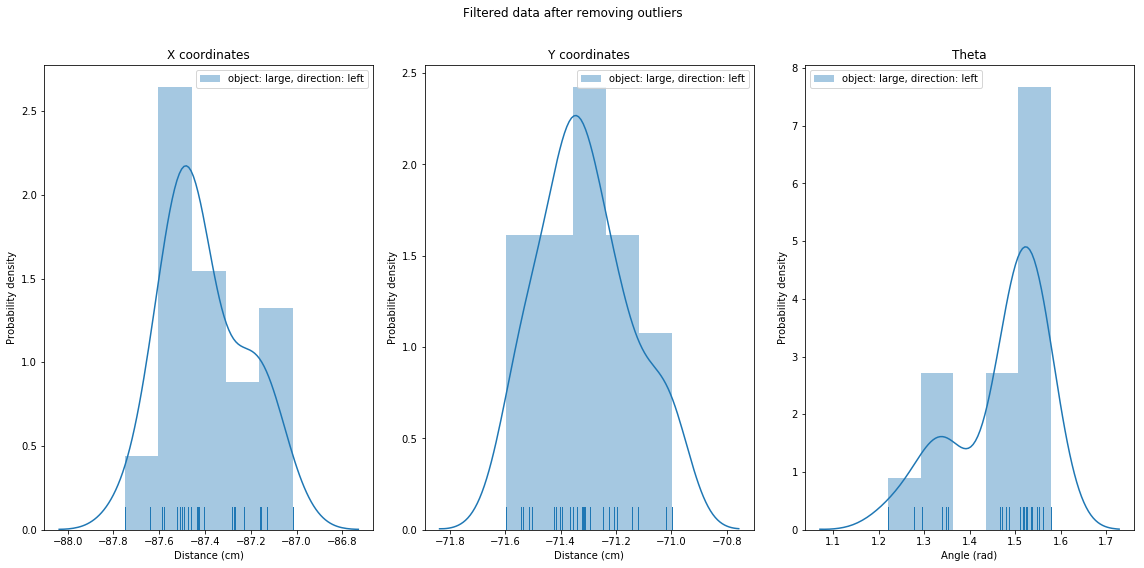
\includegraphics[width=\linewidth]{img/filtered/large_left_filtered.png}				
%							\end{subfigure}
%							\begin{subfigure}{\textwidth}
%								\centering
%								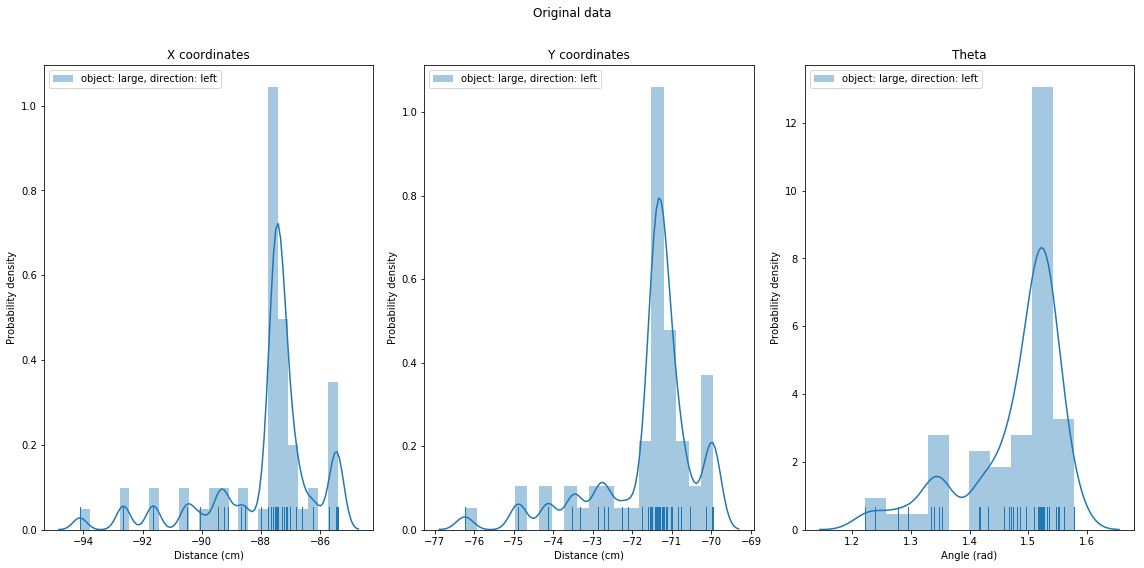
\includegraphics[width=\linewidth]{img/filtered/large_left_org.png}
%							\end{subfigure}
%							\caption{Outlier removal on large object and left run}
%						\end{figure}														
	\bibliography{references.bib}
	\bibliographystyle{plain}
\end{document}
